% Chapter Template

\chapter{Resultados} % Main chapter title

En este cap\'itulo  describiremos los datos utilizados en 	nuestros experimentos, las m\'etricas de calidad utilizadas para evaluar los resultados, la manera en la que se  utilizaron los datos y los resultados obtenidos.\\

En la secci\'on  4.1 se describen los materiales utilizados para la realizaci\'on de este trabajo final. Los tipos de dataset utilizados con las caracter\'isticas correspondientes a cada tipo de im\'agenes, dispositivos de captura, resoluci\'on de las im\'agenes, entre otras.\\

En la secci\'on 4.2  se estudian las m\'etricas de calidad utilizadas..\\

En la secci\'on 4.3 se exponen los resultados obtenidos durante el dise\'no del algoritmo..\\

En la secci\'on 4.3.1 se exponen y analizan los resultados obtenidos durante la etapa de preprocesamiento. \\

En la secci\'on 4.3.2 ..\\

En la secci\'on 4.3.3 ..\\

En la secci\'on 4.4 ..\\

En la secci\'on 4.5 ..\\



\label{Chapter4} % Change X to a consecutive number; for referencing this chapter elsewhere, use \ref{ChapterX}

%----------------------------------------------------------------------------------------
%	SECTION 1
%----------------------------------------------------------------------------------------

\section{Materiales}

Para la realizaci\'on de este trabajo final se utilizaron 3 bases de datos con im\'agenes de fondo de ojo, DRIVE, HRF, ARIA.\\

DRIVE es una base de datos a disposici\'on del p\'ublico, que consta de un total de 40 im\'agenes a color con diferentes lesiones. Las fotograf\'ias se obtuvieron a partir de un programa de cribado de la retinopat\'ia diab\'etica en los Pa\'ises Bajos. La poblaci\'on de selecci\'on consisti\'o en 453 sujetos de entre 31 y 86 a\~nos de edad. Cada imagen se ha comprimido JPEG, lo cual es una pr\'actica com\'un en los programas de cribado. De las 40 im\'agenes en la base de datos, 7 contienen la patolog\'ia, es decir, los exudados, hemorragias y cambios del epitelio pigmentario. Ver (\ref{fig:Drive_images_retinal}) para un ejemplo de una imagen patológica y una normal. Las im\'agenes fueron adquiridas mediante una c\'amara no midriática de 3 CCD Canon CR5 con un campo de $45^{\circ}$ de visi\'on (FOV). Cada i\'agen es capturada utilizando 8 bits por plano de color a 768 {x} 584 p\'ixeles. El FOV de cada imagen es circular con un di\'ametro de aproximadamente 540 p\'ixeles. El conjunto de 40 im\'agenes se dividi\'o en un conjunto de prueba y entrenamiento, ambos contienen 20 im\'agenes. Tres observadores, el primer y segundo autor y un estudiante de inform\\'atica segmentaron manualmente un n\'umero de im\'agenes. Todos los observadores fueron entrenados por un oftalm\'ologo con experiencia. El primer observador segment\'o 14 im\'agenes del conjunto de entrenamiento, mientras que el segundo observador segment\'o las otros 6 im\'agenes. El equipo de prueba fue segmentado en dos ocasiones resultando en un conjunto X e Y. El conjunto X fue segmentado tant por el primer y segundo observador (13 y 7 im\'agenes, respectivamente), mientras el conjunto Y se segmentó por completo por el tercer observador. El rendimiento de los algoritmos de segmentaci\'o de los vasos se midi\'o en la prueba. En el conjunto X los observadores marcaron 577,649 p\'ixeles como vasos y 3.960.494 como fondo (recipiente de 12,7\%). En el conjunto Y 556,532 p\'ixeles se marcaron como vasos y 3.981.611 como fondo (recipiente de 12,3\%).\\


\begin{figure}[H]
	{
	\centering
	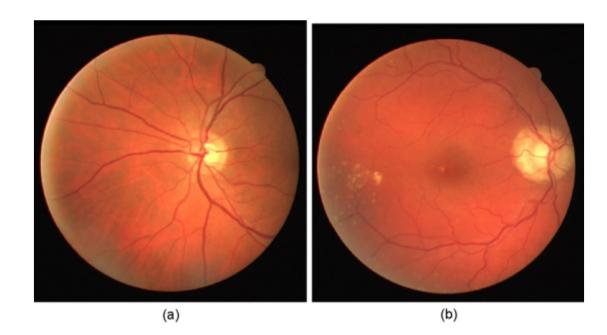
\includegraphics[width=1\textwidth]{Figures/Drive_images_retinal}
	\caption[Drive]{Im\'agen de la retina - DRIVE: (a) Retina saludable, (b) Retina con muestras patol\'ogicas.}
	\label{fig:Drive_images_retinal}
	}
\end{figure}	


HRF es una base de datos que ha sido establecida por un grupo de investigaci\'on para apoyar los estudios comparativos sobre los algoritmos de segmentaci\'on autom\'atica de im\'agenes en la retina del fondo del ojo. Es una base de datos a disposici\'on del p\'ublico, que contiene en este momento 15 im\'agenes de pacientes sanos, 15 im\'agenes de pacientes con retinopat\'ia diab\'etica y 15 im\'agenes de pacientes con glaucoma. Las im\'agenes segmentadas de los vasos est\'an disponibles para cada imagen. Tambi\'en se proporcionan las m\'ascaras, se determina el campo de visi\'on (FOV) para los conjuntos de datos particulares. Los datos est\'adar de oro son generados por un grupo de expertos que trabajan en el campo de an\'alisis de im\'agenes de la retina y los m\'edicos de las cl\'inicas oftalmol\'ogicas.\\


ARIA es una base de datos creada en 2006, en una colaboración de investigación entre  St. Paul's Eye Unit, Royal Liverpool University Hospital Trust, Liverpool, Reino Unido y el Departamento de Oftalmología, Ciencias Clínicas, Universidad de Liverpool, Liverpool, Reino Unido \cite{}. La base de datos consta de tres grupos; uno tiene 92 im\'agenes con degeneraci\'on macular relacionada con la edad, el segundo grupo tiene 59 im\'agenes con diabetes y un grupo de control se compone de 61 im\'agenes. El rastro de los vasos sangu\'ineos, la ubicaci\'on del disco \'optico y la f\'ovea est\'a marcada por dos expertos en an\'alisis de imagen como patr\'on de referencia. Las im\'agenes se capturan a una resoluci\'on de 768 {x} 576 p\'ixeles de colores RGB con 8 bits por plano de color con una c\'amara de fondo Zeiss FF450 con un campo de visi\'on de $50^{\circ}$ y se almacenan como archivos TIFF sin comprimir.\\
%-----------------------------------
%	SECTION 2
%-----------------------------------
\section{M\'etricas de calidad utilizadas}


%-----------------------------------
%	SECTION 3
%-----------------------------------

\section{Resultados obtenidos durante el dise\'no del algoritmo}

%----------------------------------------------------------------------------------------
%	SECTION 4
%----------------------------------------------------------------------------------------

\subsection{Preprocesamiento}

%----------------------------------------------------------------------------------------
%	SUBSECTION 5
%----------------------------------------------------------------------------------------

\subsection{Extracci\'on de caracter\'isticas}


%----------------------------------------------------------------------------------------
%	SECTION 5
%----------------------------------------------------------------------------------------

\subsection{Entrenamiento y clasificaci\'on}

\section{Resultado del algoritmo de segmentaci\'on propuesto}

\section{Discusi\'on}

